\documentclass[../TGMAFFIRO.tex]{subfiles}

\begin{document}
In order to explain the likelihood of certain random events, we must first define what we mean by \textit{randomness}, specify which events are being referred to, and express, in a mathematical sense, the possibility of any such event. With this in mind, we dedicate this chapter to gradually build the tools that will later be required to \textit{make sense} of random events and further develop a theory to model the dynamics of assets such as stocks and currencies.\\

We begin by formalizing \textit{measurable spaces} and proof important results of fundamental importance throughout this work.

\section{Measurable Spaces}

\begin{definition}[\textbf{$\salg$}]\label{def:sigma_algebra}
	Let $\Omega$ be a set of points $\omega$. A system $\salgF$ of subsets of $\Omega$ is a $\salg$ if:
	\begin{enumerate}
		\item $\Omega \in \salgF$;
		\item If $\{A_n\}_{n\geq 1} \in \salgF \Rightarrow \bigcup_{k=1}^{\infty} A_k \in \salgF$; and
		\item If $A \in \salgF \Rightarrow A^\mathsf{c} \in \salgF$.
	\end{enumerate}
\end{definition}

\begin{remark}
	For $\{A_n\}_{n\geq 1} \in \salgF$ then, definition \ref{def:sigma_algebra} is equivalent to say that
	\begin{equation*}
		\text{If } \{A_n\}_{n\geq 1} \in \salgF \Rightarrow \bigcap_{k=1}^{\infty} A_k \in \salgF.
	\end{equation*}
\end{remark}

\begin{proof}
	By the generalized form of De Morgan's laws, $(\bigcap_k A_k)^\mathsf{c} \equiv \bigcup_k A_k^\mathsf{c}$. Since $A_k \in \salgF \ \forall \ k$ then, by definition,  $A_k^\mathsf{c} \in \salgF \ \forall \ k$ which implies  $\bigcup_k A_k^\mathsf{c}$ and this complement is also in $\salgF$
\end{proof}

\begin{definition}\label{generated_sigma_algebra}
	let $\emptyset \neq A$ a set of elements of $\Omega$ . The $\salg$ generated by $A$, denoted by $\sigma(A)$, is the set
	\begin{equation}
		\sigma(A) := \bigcap\{\salgF : \salgF \text{ is sigma algebra, and } A \subseteq \salgF \}.
	\end{equation}

\end{definition}

Defintion \ref{generated_sigma_algebra} is the smallest $\salg$ that cointains $A$. This definition is useful in the construction of one particular $\salg$ of subsets of $\RNums$.\\

Consider the collection of open intervals $(a,b) \in \RNums$. For every $a \leq b$, the smallest $\salg$ generated by this collection is known as the Borel $\salg$ of subsets of $\RNums$.

\begin{definition}[\textbf{The Borel $\salg$}]\label{def:borel_sigma_alg}
		\begin{equation}
			\borelsalg := \sigma\{(a,b) \subseteq \RNums:a\leq b\}.
		\end{equation}
\end{definition}

Definition \ref{def:borel_sigma_alg} is the smallest $\salg$ that contains all open intervals in the real line. Furthermore, it can be proven that $[a, b]$, $(a,\infty)$, $(-\infty, b)$, $[a, b)$, $(a, b]$ are all elements in $\borelsalg$.\\

Concerning the set of elements $\Omega$, equipped with a $\salg \ \salgF$, yields a crucial definition that will formalize an abstract space in which we can further develop a theory.

\begin{definition}[\textbf{Measurable Space}] \label{def:measurable_space}
	If $\salgF$ is a $\salg$ of subsets of $\Omega$, $(\Omega, \salgF)$ is said to be a measurable space. If $A$ is a set in $\salgF$, we say that $A$ is $\salgF$-measurable ---or measurable with respect to (w.r.t.) $\salgF$---
\end{definition}

Definition \ref{def:measurable_space} urges an auxiliary way to make sense of the information provided by $(\Omega, \salgF)$. Concretely, we now define a way to fathom any abstract measurable space.

\begin{definition}[\textbf{Measure}]
	Let $\bar{\mathbb R} := \mathbb R \cup \{-\infty, \infty\}$ be the extended real line and let $(\Omega, \salgF)$ be a measurable space. It is said that a function $\mu: \salgF \rightarrow \bar{\mathbb R}$ is a measure over $(\Omega, \salgF)$ if
	\begin{enumerate}
		\item $\mu(\emptyset) = 0$;
		\item $\mu(A) \geq 0\ \forall \ A \in \salgF $; and
		\item $\mu$ is $\sigma$-additive: If $\{A_k\}_{k=1}^{\infty}$ is a set of disjoint events in $\salgF$ ($A_i \cap A_j = \emptyset \ \forall \ i \neq j$), 
		\begin{equation*}
			\bigcup_{k=1}^{\infty} \mu(A_k) = \mu(\sum_{k=1}^{\infty} A_k).
		\end{equation*}
	\end{enumerate}
\end{definition}


If the last definition holds true for a given $\mu$ inside $(\Omega, \salgF)$, then $\MeasureSpace{\mu}$ is said to be a \textbf{measure space}. Thus, for any $A\in\salgF$, $\mu(A)$ is the measure of $A$.\\

 Furthermore, if $\mu(\Omega) < \infty$ then, $\mu$ is said to be a finite measure. Lastly, if  $\mu(\Omega) = 1$, then $\mu$ is said to be a probability, which we denote $\Pm \equiv \mu$. Consequently, $\ProbSpace$ is said to be a \textbf{probability space}. We formalize this last definition as follows:

\begin{definition}[\textbf{Kolmogorov's Axiom System}]\label{def:kolmogorov_axions}
	An ordered triple $\ProbSpace$ where
	\begin{enumerate}
		\item $\Omega$ is a set of points $\omega$;
		\item $\salgF$ is a $\salg$ of subsets of $\Omega$; and
		\item $\mathbb P$ is a probability on $\salgF$,
	\end{enumerate}
	is called a \textbf{probability space} or \textbf{model} (of an experiment)
\end{definition}

As a result of definition \ref{def:kolmogorov_axions}, if $\ProbSpace$ is a probability space and $A \in \salgF$, it is said that $\Pm(A)$ is the \textit{probability of the event A}.

\section{Random Variables}
For any given probability space $\ProbSpace$, $\Omega$ is defined to be any abstract space. To overcome the problem of abstraction, it is desirable to find a mapping from elements in $\Omega$ to the more convenient $\RNums$, in the sense that, measurements on the real line, if mapped correctly, may become easier to interpret. In view of the coveted property of interpretability, we define a mapping $\Omega\to\RNums$ that is consistent with the theory developed so far.

\begin{definition}\label{def:rvar}
	Let $\ProbSpace$ be a probability space. The function $X: \Omega \rightarrow \RNums$ it is defined an $\salgF$-measurable function or a \textbf{random variable} if
	\begin{equation}
		X^{-1}(B) = \{\omega \in \Omega \ | \ X(\omega) \in B\} \in \salgF \ \ \forall \ \ B \subseteq \borelsalg.
	\end{equation}
\end{definition}

% dovetail.- verb: to join or fit together compactly or harmoniously.
With definition \ref{def:rvar}, measurements over $\Omega$ dovetail with an element of order. Consequently, it becomes natural to define the following:

\begin{definition}\label{dist_func}
	Consider the event $\{X \leq x\} := X^{-1}(-\infty, x]$. The function $F_X: \RNums \rightarrow [0, 1]$ defined as:
	\begin{equation}
		F_X(x) := \Pm\{X \leq x\},
	\end{equation}
	is known as the \textbf{distribution function} of the random variable $X$.
\end{definition}

Furthermore, a probability distribution function has the following properties:
\begin{enumerate}
	\item For $x \leq y$ then, $F_X(x) \leq F_X(y)$;
	\item $\lim\limits_{x\to\infty} F_X(x) = 1$ and $\lim\limits_{x\to - \infty} F_X(x) = 0$; and
	\item $F_X$ is right-continuous, meaning that $\lim\limits_{y\to x^+} F_X(y) = F_X(x)$ for every $x \in \RNums$.
\end{enumerate}

\begin{definition}
	A random variable $X$ is said to be \textbf{absolutely continuous} if there exists a nonnegative borel-measurable function $f: \RNums\rightarrow\RNums$ such that 
	\begin{equation}
		F_X(x) = \int_{-\infty}^{x} f(t) dt.
	\end{equation}
\end{definition}


The function $f$ is known as the \textbf{probability density function} (p.d.f.) of the random variable $X$. Perhaps one of the most well known probability density functions, and a crucial tool for this work, is the p.d.f. of the normal distribution:

\begin{equation}\label{eq:normal_distribution}
	f(x|\mu, \sigma^2) = \frac{1}{\sqrt{2\pi\sigma^2}}e^{-\frac{(x - \mu)^2}{2\sigma^2}}.
\end{equation}

\begin{figure}[h]
	\centering
	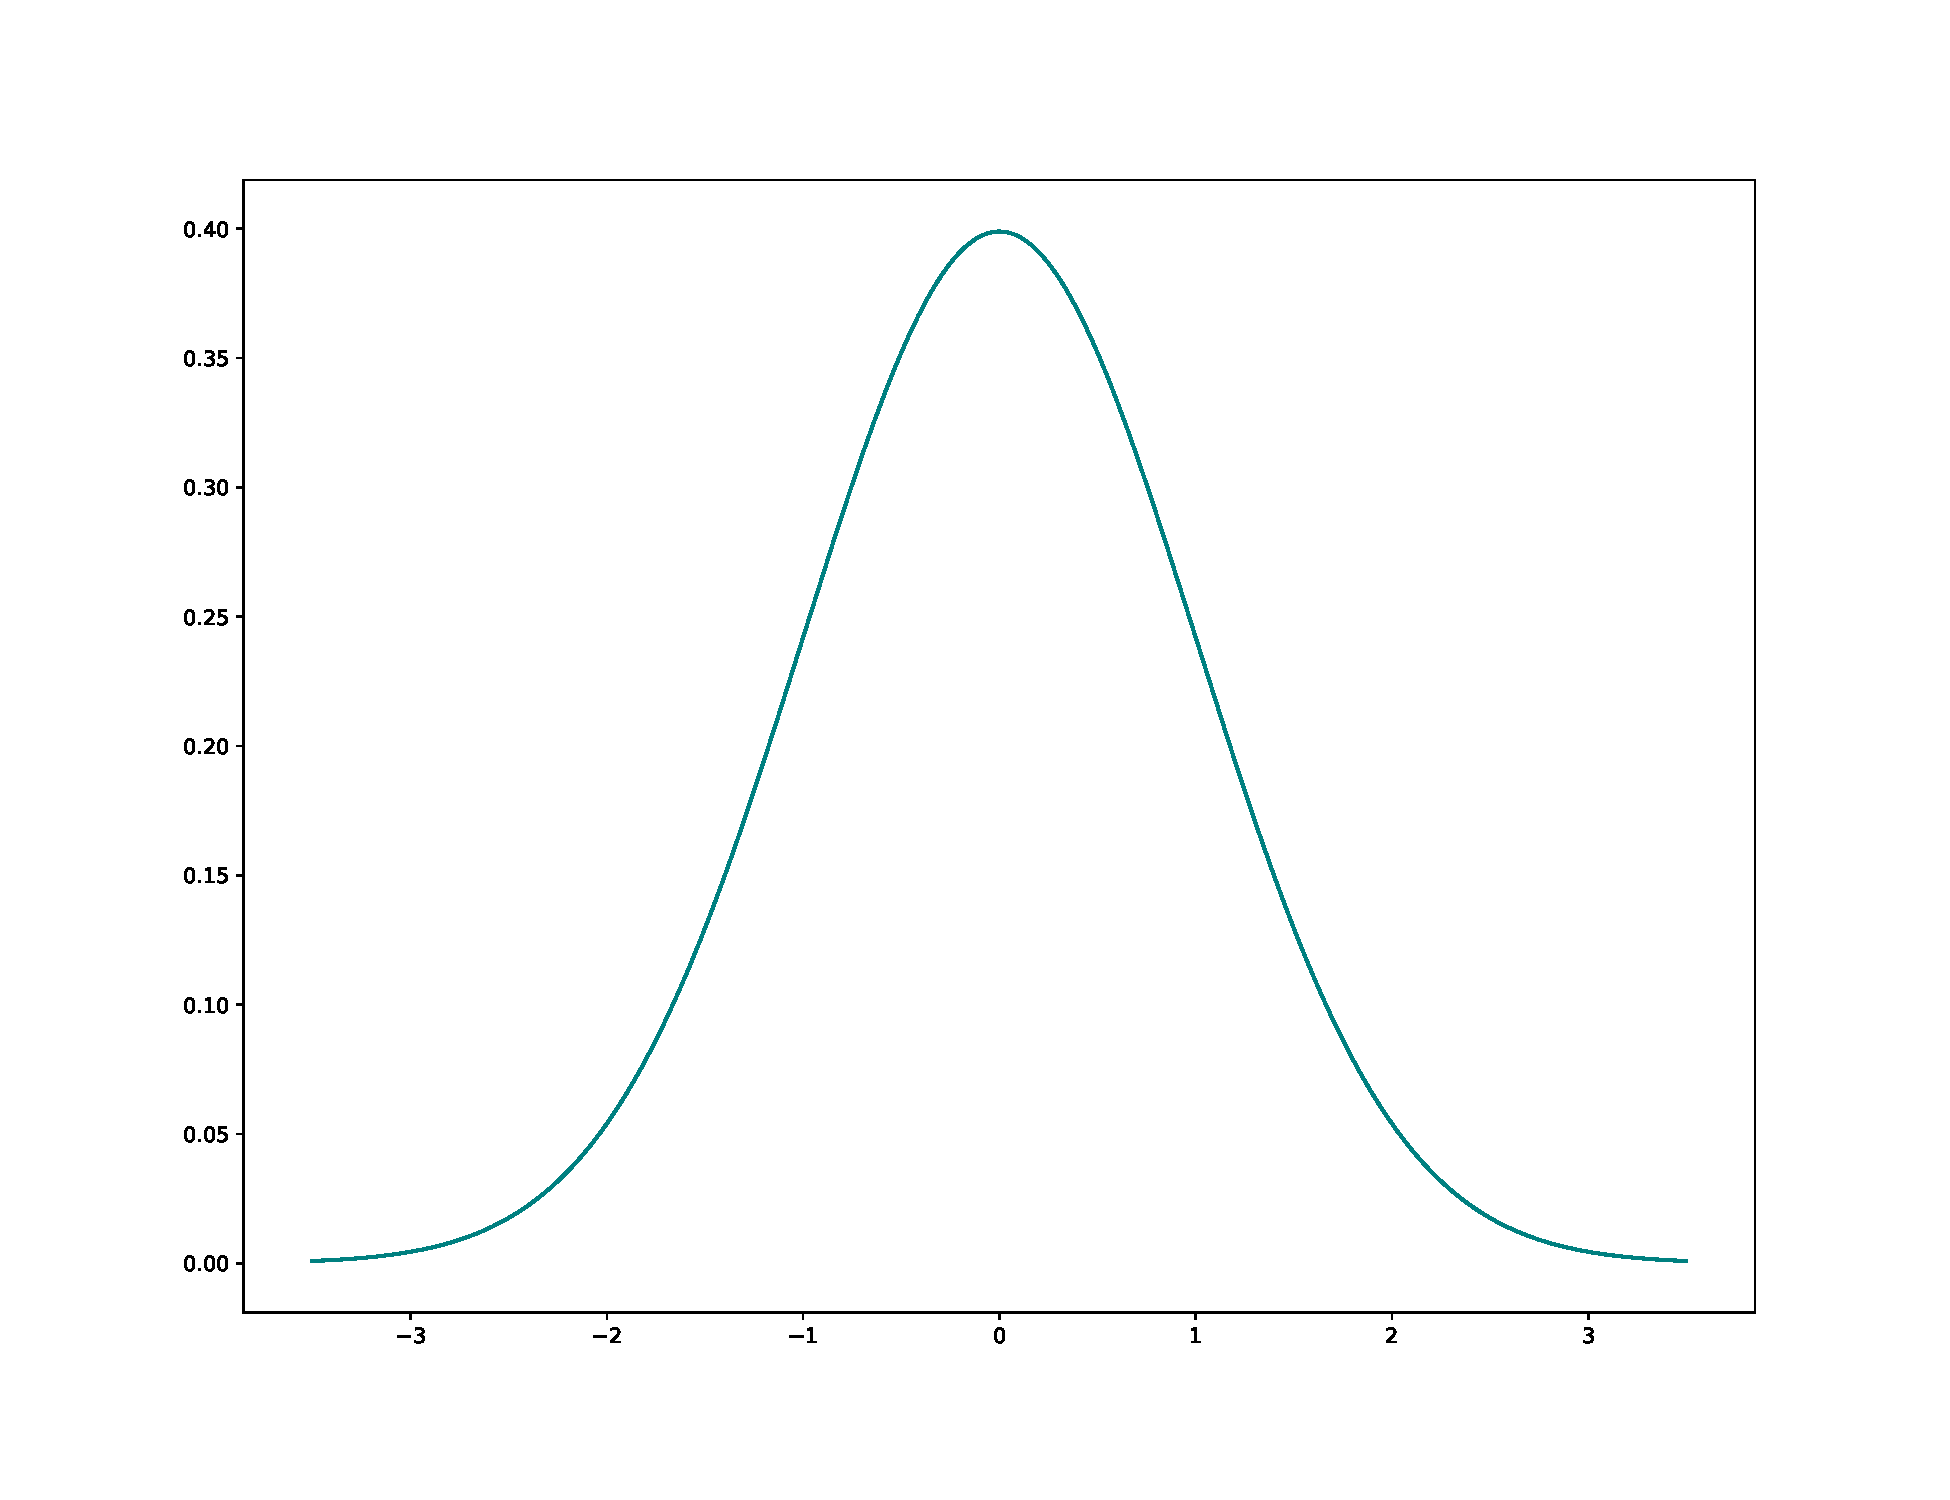
\includegraphics[width=0.6\textwidth]{../images/normal_distribution}
	\caption{Probability Density Function of a Normal Distribution $\phi(x|0,1)$.}
	\label{fig:normal_distribution}
\end{figure}

We denote the normal distribution as $\mathcal{N}(\mu, \sigma^2)$. Also, if $X$ normally distributed with parameters $\mu$ and. $\sigma^2$, we write $X \sim N(\mu, \sigma^2)$.


\section{Lebesgue Integrals and Expectations}
We now present the key ideas behind Lebesgue integration. As we shall later see, random movements over time (e.g. a stock or FX exchange rate) can be modeled as the sum of infinitesimal random changes. A thorough understanding of the ideas behind integration allow us to more easily understand the machinery for much more complex, stochastic models. In addition, Lebesgue integrals pave the way to the mathematical expectation, a core idea in the theory of probability.\\

We start the motivation of a Lebesgue integral by defining the most basic class of measurable functions.

\begin{definition}
	Let $\MeasureSpace{\mu}$ be a measure space and $X: \Omega \to \RNums$ an $\salgF$-measurable function. Denote $\ind_A(\omega)$ the indicator function of $\omega$ in a set $A$. That is,
	\[
	\ind_A(\omega) = 
		\begin{cases}
			1 & \omega \in A \\
			0 & \omega \notin A
		\end{cases}
	\]
	To simplify the notation, we will also denote $\ind_A(\omega)$ as $\ind_A$.
	We define the \textbf{Lebesgue integral} of $\ind_A$ w.r.t. $\mu$ as
	\begin{equation}
		\int_\Omega \ind_A(\omega) d\mu(\omega) := \mu(A).
	\end{equation}
	
\end{definition}

\begin{definition}
	Let $(\Omega, \salgF)$ a measurable space and $X$ an $\salgF$-measurable function. It is said that $X$ is a \textbf{simple function} if it takes only a unique finite number of values $\{x_i\}_{i=1}^{n} \in \RNums$. Then, $X$ can be written as
	\begin{equation}
		X(\omega) = \sum_{i=1}^{n}x_i\ind_{A_i}.
	\end{equation}
	Where,
	\[
		A_i := \{\omega \in \Omega | X(\omega) = x_i\} \ \forall \ i = 1, \ldots, n
	\]
\end{definition}

\begin{definition}
	let $X$ be a simple function, we define the integral of $X$ w.r.t. $\mu$ as:
	\begin{equation}
		\int_\Omega X(\omega) d\mu(\omega) := \sum_{i=1}^{n}x_i\mu(A_i).
	\end{equation}
\end{definition}

%% TODO: add theorem (proof?) that that any continuous function can be approximating as the limit of simple functions

\begin{theorem}
	If $f:\RNums\to[0, \infty]$ is measurable, then there exist a collection of real-valued simple functions $\{f_i\}_{i\geq 0}$ on $f$ such that $0 \leq f_1 \leq \ldots \leq f$ and $f_n \to f$ pointwise.
\end{theorem}

\begin{proof}
	For an overview of the proof, see \aycite{fairchild}.
\end{proof}

%% Approximation by Simple Functions %%
\begin{figure}[h]
	\centering
	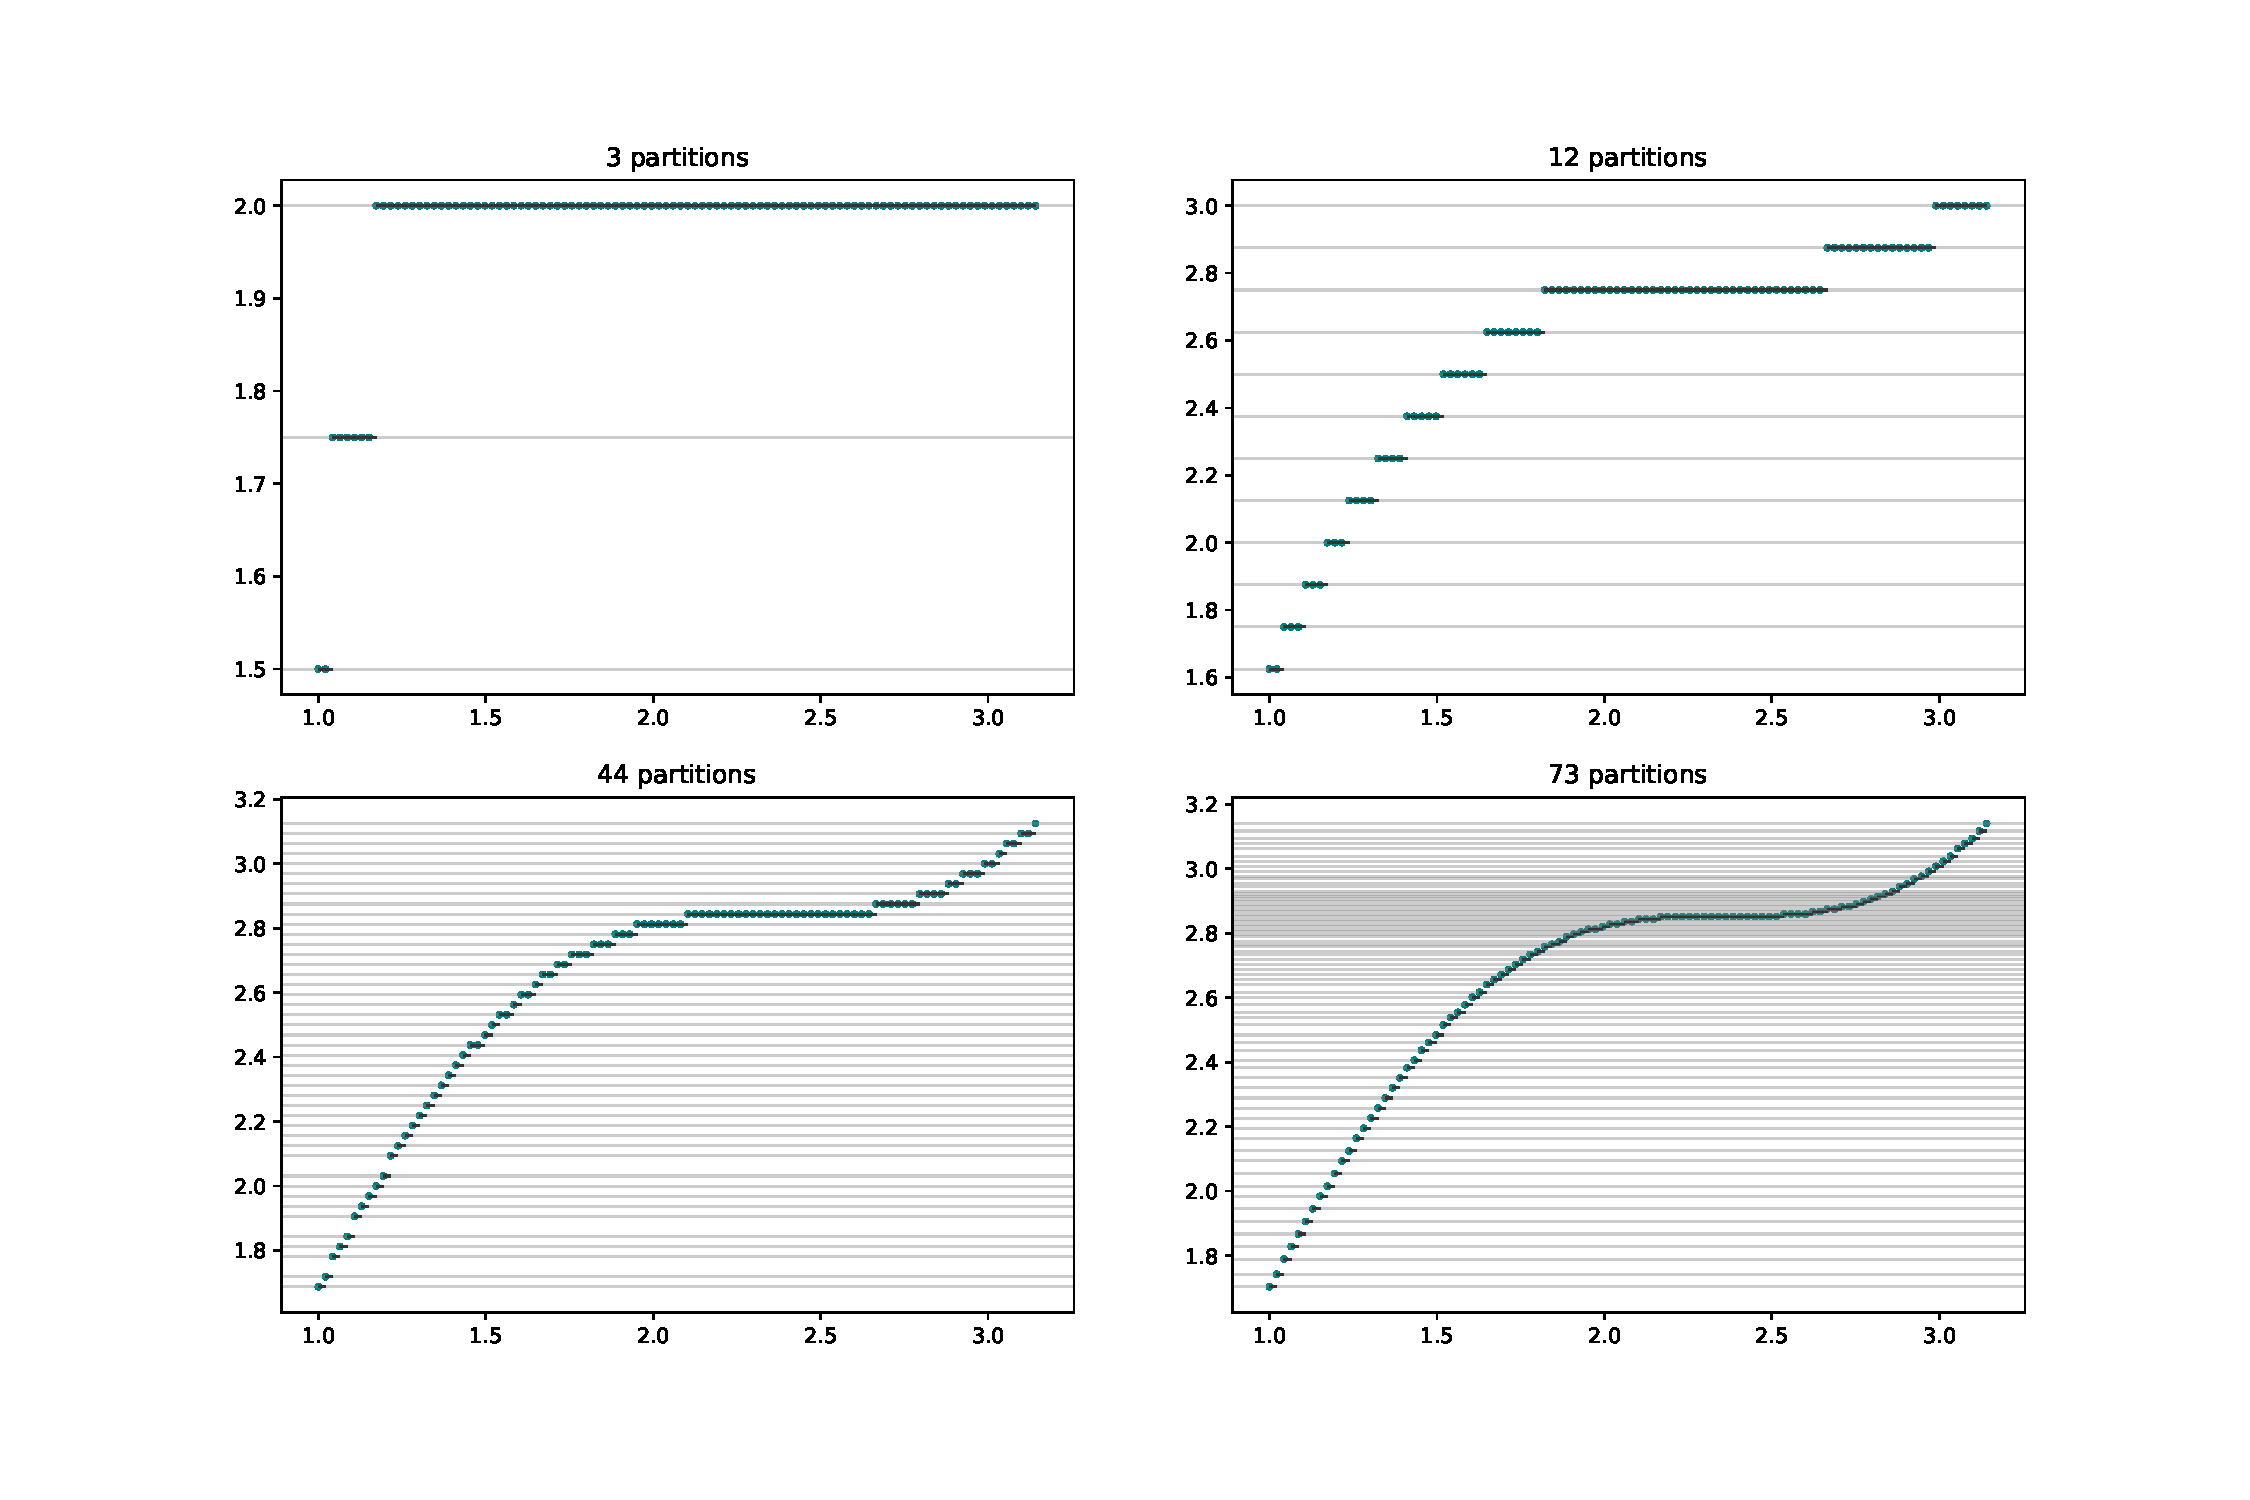
\includegraphics[width=0.9\textwidth]{../images/simple_sine.pdf}	
	\caption{Approximation to the Borel-measurable function $\sin^2(x) + x$ via a sequence of simple functions}
	\label{fig:simple_approx_sine}
\end{figure}

%% Nonnegative lebesgue measure for nonnegative simple functions
\begin{proposition} \label{prop:nnlmsf}
	Let $X$ be a nonnegative simple function defined on a measurable space $\MeasureSpace{\mu}$ in which $\mu(\Omega) < \infty$. Then,
	\begin{equation}
		\int_\Omega X d\mu \geq 0.
	\end{equation}
\end{proposition}

\begin{proof}
	Since $X$ is a nonnegative simple function, it follows that
	\[
	\int_\Omega X d\mu = \sum_{i=1}^n x_i \mu(A_1),
	\]
	where $x_i \geq 0 \ \forall \ i \in \{1, \ldots, n\}$. Also, $\mu(A_i) \geq 0 \ \forall \ A_i \in \salgF$.
\end{proof}

\begin{theorem}
	If $X$ and $Y$ are two non-negative simple functions and $\alpha, \beta \geq 0$,
	\begin{equation}
		\int_\Omega (\alpha X + \beta Y) d\mu = \alpha\int_\Omega X d\mu + \beta\int_\Omega Y d\mu.
	\end{equation}
	
	If $X \leq Y$ then,
	\begin{equation}
		\int_\Omega X \leq \int_\Omega Y.
	\end{equation} 
\end{theorem}

\begin{proof}
	Let, $X = \sum_{i=i}^{n}x_i\ind_{A_i}$ and $Y = \sum_{j=1}^{m}y_i\ind{B_i}$. Note that $\bigcup_i A_i = \bigcup_j B_j = \Omega$. Also, $\ind_A = \sum_{i=1}^{n}\ind_{A_i}$ since $\{A_i\}$, by definition of the Lebesgue integral, is a set of disjoint elements. Then, $X$ and $Y$ can be written as
	\begin{align*}
		X	&= \sum_{i=1}^{n}\ind_{A_i\cap\Omega} \\
			&= \sum_{i=1}^{n}\ind_{A_i\cap\left(\cup B_j\right)}\\
			&= \sum_{i=1}^{n} \sum_{j=1}^{m} x_i \ind_{A_i \bigcap B_j}.
	\end{align*}
	
	Similarly for $Y$,
	\begin{align*}
		Y	&= \sum_{j=1}^{m} \sum_{i=1}^{n} y_i \ind_{B_j \bigcap A_i} \\
			&= \sum_{i=1}^{n} \sum_{j=1}^{m} y_i \ind_{A_i \bigcap B_j}.
	\end{align*}
	
	Then,
	\begin{align*}
		\alpha X + \beta Y  &= \alpha \sum_{i=1}^{n} \sum_{j=1}^{m} x_i \ind_{A_i \bigcap B_j} + \beta \sum_{i=1}^{n} \sum_{j=1}^{m} y_i \ind_{A_i \bigcap B_j} \\
				&= \sum_{i=1}^{n} \sum_{j=1}^{m} (\alpha x_i + \beta y_i) \ind_{A_i \bigcap B_j}.
	\end{align*}
	
	Now, 
	\begin{align*}
		\int_\Omega\alpha X+\beta Y &= \sum_{i=1}^{n} \sum_{j=1}^{m} (\alpha x_i + \beta y_i) \mu(A_i \cap B_j) \\
		&= \alpha \sum_{i=i}^{n}\left(\sum_{j=1}^{m} x_i \mu(A_i\cap B_j) \right) + \beta \sum_{j=1}^{m}\left(\sum_{i=1}^{n} x_i \mu(A_i\cap B_j) \right)\\
		&= \alpha \sum_{i=i}^{n}x_i \mu(A_i) + \beta\sum_{j=1}^{m} y_i \mu(B_i) \\
		&= \alpha \int_\Omega X d\mu + \beta\int_\Omega Y d\mu.
	\end{align*}
	
	We now set out to prove the monotonicity property for nonnegative simple functions. 
	Let $X \leq Y$ then, $Y - X \geq 0$ is an $\salgF$-measurable function. By proposition \ref{prop:nnlmsf},
	\begin{equation}
		Y - X \geq 0 \implies \int_\Omega (Y - X) d\mu \geq 0.
	\end{equation}	
\end{proof}

\begin{definition}
	For any nonnegative function $X$, we define the integral of $X$ w.r.t. a measure $\mu$ as
	\begin{equation}\label{def:lebesgue_integral}
		\int_\Omega Xd\mu := \sup\left\{\int_\Omega h d\mu \ | \ 0 \leq h \leq X \text{, $h$ is simple}\right\}.
	\end{equation}
\end{definition}

If $X$ is any measurable function, we define the positive and negative parts of $X$ as:
\begin{align}
	X^+ := \max\{X(\omega), 0\} \text{; and}\\
	X^- := \max\{-X(\omega), 0\}.
\end{align}

Thus, $X = X^+ - X^-$, and $|X| = X^+ + X^-$. Since both parts of $X$ are positive, their integrals are well defined.\\

If both $\int_\Omega X^+ d\mu$ and $\int_\Omega X^- d\mu$ are finite, we say that $X$ is integrable w.r.t. $\mu$. By linearity, 

\begin{equation}
	\int_\Omega X d\mu = \int_\Omega X^+ d\mu - \int_\Omega X^- d\mu.
\end{equation}

And,

\begin{equation}
	\int_\Omega |X| d\mu = \int_\Omega X^+ d\mu + \int_\Omega X^- d\mu.
\end{equation} \\

We will denote by $L_1 \equiv L_1\MeasureSpace{\mu}$ the family of integrable functions w.r.t. $\mu$. Note that $X \in L_1$ if and only if $|X| \in L_1$. i.e.,

\begin{equation}
	\int_\Omega |X| d\mu = \int_\Omega X^+ d\mu + \int_\Omega X^- d\mu < \infty.
\end{equation}

If $A \in \salgF$, we define
\begin{equation}
	\int_A X d\mu := \int_\Omega X \ind_A d\mu.
\end{equation}

\begin{proposition} \label{prop:lebesgue_integral_props}
	For any $X$, $Y$ $\salgF$-measurable functions in $L_1$; $A$, $B$ members of $\salgF$, it can be shown that:
	\begin{equation}\label{prop:integral_positive_measure}
		X \geq 0 \implies \int_\Omega X d\mu \geq 0. \\
	\end{equation}
	
	If $X \leq Y$ (monotonicity),
	\begin{equation}
		\int_\Omega X d\mu \leq \int_\Omega Y d\mu.
	\end{equation}
	
	If $A \subseteq B$ and $X \geq 0$,
	\begin{equation}
		\int_A X d\mu \leq \int_B X d\mu.
	\end{equation}
	
	If $\alpha$, $\beta$ $\in \RNums$ (linearity),
	\begin{equation}
	\int_\Omega (\alpha X + \beta Y) d\mu = \alpha \int_\Omega X d\mu + \beta \int_\Omega Y d\mu.
	\end{equation}
\end{proposition}

%TODO Add hints in how to solve them (a generalization of integrals of simple functions)

\begin{theorem} \label{th:salg-lebesgue-int}
	Let $\MeasureSpace{\mu}$ be a measurable space, and $X$ a nonnegative $\salgF$-measurable function. If $X: \Omega \to \RNums$, the mapping from $\Omega \to [0, \infty]$ given by $A \to \int_A f d\mu$ is $\sigma$-additive, i.e.
	\begin{equation}
		\int_A X d\mu = \sum_{i=1}^{\infty}\int_{A_i} X d\mu.
	\end{equation}
	For disjoint sets $\{A_i\}_{i\geq1}$
\end{theorem}

For a proof of theorem \ref{th:salg-lebesgue-int} see \aycite{applebaum}. Consider \ref{def:lebesgue_integral}, \ref{prop:integral_positive_measure}, together with theorem \ref{th:salg-lebesgue-int}. It is then clear that the Lebesgue integral for random variables $X \in \ProbSpace$ such that $X(\omega) \geq 0 \ \forall \ \omega \in \Omega$ is then a measure defined over $(\RNums, \borelsalg)$. This last is followed by a corollary that will aid in the result of one of the fundamental theorems of integration and convergence. 

\begin{corollary} \label{cor:partition_limit_integral}
	Let $X: \Omega \to \RNums$ a nonnegative measurable function and $\{E_n\}_{n\geq 1}$ a sequence of sets in $\Omega$ such that $E_n \subseteq E_{n+1}$ for every $n \in \mathbb{N}$. Denote $E = \bigcup_{n=1}^{\infty} E_n$. Then,
	\begin{equation}
		\int_E X d\mu = \lim_{n\to \infty} \int_{E_n} X d\mu.
	\end{equation}
\end{corollary}

\begin{proof}
	Denote $A_1$ = $E_1$, and $A_n = E_n - E_{n-1} \ \forall \ n \geq 2$. The set $\{A_n\}_n$ is a sequence of disjoint sets. Note that, $E = \bigcup_{i=1}^\infty A_i$ and $E_n = \bigcup_{i=1}^n A_i$ $\forall \ n \in \mathbb{N}$.\\
	
	By theorem \ref{th:salg-lebesgue-int},
	
	\begin{align*}
		\int_E X d\mu &= \int_{\bigcup_{i=1}^{\infty} A_i} X d\mu \\
		&= \sum_{i=1}^{\infty} \int_{A_i} X d\mu \\
		&= \lim_{n\to\infty} \sum_{i=1}^{n} \int_{A_i} X d\mu \\ 
		&= \lim_{n\to\infty} \int_{\bigcup_{i=1}^{n} A_i} X d\mu \\
		&= \lim_{n\to\infty} \int_{E_n} X d\mu.
	\end{align*}
\end{proof}


\begin{theorem}[\textbf{Monotone Convergence Theorem}]
Let $\{X_n\}_{n\geq 1}$ be a sequence of nonnegative functions where $X_i: \Omega \to \RNums$ such that $X_n \leq X_{n+1}$ $\forall \ n \in \mathbb{N}$. Let $X$ be another random variable such that $X_n \to X$ then,
\begin{equation}
	\int_\Omega X d\mu = \lim_{n\to \infty} \int_\Omega X_n d\mu.
\end{equation}
\end{theorem}

\begin{proof}
	Since $X = \sup_{n\in \mathbb{N}}X_n$, by monotonicity,
	\begin{equation*}
		\int_\Omega X_1 d\mu \leq \int_\Omega X_1 d\mu \leq \ldots \leq \int_\Omega X d\mu.
	\end{equation*}
	Thus,
	\begin{equation*}
		\lim_{n\to\infty}\int_\Omega X_n d\mu \leq \int_\Omega X d\mu.
	\end{equation*}
	
	To show the reverse inequality, let $0 \leq h \leq X$ a a simple function and let $c \in (0,1)$. Denote $A_n = \{\omega\in\Omega \ | \ X_n(\omega) \geq c\cdot h(\omega)\}$.\\
	
	Since $\{X_n\}_{n\geq 1}$ is a sequence of nondecreasing functions, $A_n \subseteq A_{n+1}$ $\forall$  $n\in\mathbb{N}$. One final property of $\{A_n\}$ is the fact that $\bigcup_nA_n = \Omega$.	This last property can be shown by noticing that each $A_n$ has two possible outcomes to determine whether any $\omega\in\Omega$ is inside $A_n$:\\
	
	Consider $h(\omega)=0$. In that case, any $A_k = \{\omega\in\Omega \ | \  X_k(\omega) \geq 0\}$ will capture every element $\omega$. Consider now $h(\omega) \neq 0$. In this case, we do not know for which $k\in\mathbb{N}$ will $c\cdot h \leq X_k$, nonetheless, since $X_n \to X$, for some $k\in\mathbb N$, $X_k(\omega) \leq c\cdot h(\omega)$.
	
	By proposition \ref{prop:lebesgue_integral_props},
	\begin{equation}
		\lim_{n\to\infty}\int_\Omega X_n d\mu \geq \int_\Omega X_n d\mu \geq \int_{A_n} X_n d\mu \geq \int_{A_n} c\cdot h d\mu.
	\end{equation}
	
	As $A_n$ is an increasing sequence,
	\begin{equation}
		\lim_{n\to\infty}\int_\Omega X_n d\mu \geq \lim_{n\to\infty}\int_{A_n} c\cdot h d\mu.
	\end{equation}
	
	Taking account of the linearity property for Lebesgue integrals and corollary \ref{cor:partition_limit_integral},
	\begin{equation}
  		\lim_{n\to\infty}\int_{A_n} c\cdot h d\mu = c\int_{\Omega} h d\mu.
	\end{equation}
	
	Choosing an arbitrary $c \in (0,1)$, set $c= 1 - \frac{1}{k}$ and let $k\to\infty$,
	\begin{equation}
  		\lim_{n\to\infty}\int_\Omega X_n d\mu \geq \lim_{k\to\infty} \left(1 - \frac{1}{k}\right)\int_{\Omega} h d\mu = \int_{\Omega} h d\mu.
	\end{equation}
	
	Choosing an arbitrary $h$, we find that
	\begin{equation}
  		\lim_{n\to\infty}\int_\Omega X_n d\mu \geq \sup\left\{\int_{\Omega} h d\mu\right\} = \int_\Omega X d\mu.
	\end{equation}
\end{proof}

% TODO: Must writing about convergence a.e. and convergence in measure

\begin{proposition} \label{prop:convergence_ae_measure}
	If $f_n \to f$ a.e. then $f_n \to f$ in measure.
\end{proposition}

\begin{theorem}[\textbf{Bounded Convergence Theorem}]
	If the sequence $\{f_n\}_{n\geq 1}$ of measurable functions is uniformly bounded and if $f_n \to f$ in measure then,
	\begin{equation}
		\lim_{n\to\infty} \int_\Omega f_n = 	\int_\Omega \lim_{n\to\infty} f_n d\mu = \int_\Omega f d\mu
	\end{equation}
\end{theorem}

\begin{proof}
	First we note that
	\[
		|\int f_n d\mu - \int f d\mu| = |\int (f_n - f) d\mu| \leq \int| (f_n - f) | d\mu.
	\]
	We now denote $g_n := f_n - f$. Thus, we are left to show that if $g_n \to 0$ in measure and $|g_n| \leq M$ then $\int |g_n| d\mu \to 0$. To prove this, consider the following partition
	\[
		\int|g_n| d\mu = \int_{|g_n| \leq \epsilon}|g_n| d\mu + \int_{|g_n| > \epsilon}|g_n| d\mu \ \forall \ \epsilon > 0.
	\]
	Where,
	\[
		\int_{|g_n| \leq \epsilon} |g_n| d\mu \leq \epsilon,
	\]
	and
	\[
		\int_{|g_n| > \epsilon} f_n d\mu \leq M\int_{|g_n| > \epsilon} d\mu = M\cdot\mu(\{\omega : |g_n(\omega)| > \epsilon\}).
	\]
	Then,
	\begin{equation}
		\int g_n d\mu \leq \epsilon + M\cdot\mu(\{\omega : |g_n(\omega)| > \epsilon\}).
	\end{equation}
	Taking limits we find that that
	\[
		\lim_{n\to\infty} |g_n| d\mu \leq \epsilon
	\]
	since $\{\omega : |g_n(\omega)| > \epsilon\}$ converges to an empty set as $n\to\infty$. This completes the proof since $\epsilon > 0$ is as small as desired.
\end{proof}

\begin{theorem}[\textbf{Fatou's Lemma}]\label{th:fatous_lemma}
If $\{f_n\}_{n\geq 1}$ is a sequence of nonnegative measurable functions such that $f_n \to f$ in measure. Then,
\begin{equation}
	\int\lim_{n\to\infty}\inf f_n d\mu = \int f d\mu \leq \lim_{n\to\infty}\inf\int f_n d\mu
\end{equation}
\end{theorem}

\begin{proof}
	Let $0 \leq g \leq f$, and define $h_n:= \min\{f_n, g\}$ then,
	\[
		\lim_{n\to\infty} h_n = g,
	\]
	since $h_n$ tends to $g$ a.e., by proposition \ref{prop:convergence_ae_measure}, $h_n \to g$ in measure. It follows by the bounded convergence theorem that
	\begin{equation}
		\lim \int h_n d\mu = \int \lim h_n d\mu = \int g d\mu
	\end{equation}
	Now, 
	\[
		\int h_n d\mu = \int \min\{g, f_n\} d\mu \leq \int f_n d	\mu \ \forall \ n.
	\]
	It follows that
	\[
		\int h_n d\mu \leq \inf\int f_n d\mu.
	\]
	Finally, taking limits,
	\[
		\lim_{n\to\infty} \int h_n d\mu = \int g d\mu \leq \lim_{n\to\infty}\inf \int f_n d\mu
	\]
	As $0 \leq g \leq f$ is arbitrary, choosing $g = f$ concretes the proof.
\end{proof}

\begin{theorem}[\textbf{Dominated Convergence Theorem}]
If the sequence $\{f_n\}_{n\geq 1}$ is such that $f_n \to f$ in measure, and $|f_n| \leq g$ for measurable $g$, and all $n$, $\omega$ then,
\begin{equation}
	\lim_{n\to\infty}\int f_n d\mu = \int \lim_{n\to\infty} f_n d\mu  = \int f d\mu
\end{equation}
\end{theorem}

\begin{proof}
	Let $\{f_n\}$ the sequence of measurable simple functions that converge to $f$ in measure. Consider measurable $g$ such that $0 \leq f_n \leq g$. Then, $g + f_n \to g + f$, $g - f_n \to g + f$ in measure. By Fatous's Lemma (\ref	{th:fatous_lemma}),
	\[
		\int(g + f) d\mu \leq \lim_{n\to\infty}\inf\int(g + f_n) d\mu
	\]	
	As $g$ is integrable, and considering the linearity of the integral, we can write
	\[
		\int f d\mu \leq \lim_{n\to\infty}\inf\int f_n d\mu.
	\]
	Similarly, for $g - f_n$ we write
	\[
		\int(g - f) d\mu \leq \lim_{n\to\infty} \inf \int (g - f_n) d\mu.
	\]
	Then,
	\[
		\int f d\mu \geq \lim_{n\to\infty} \inf \int f_n d\mu
	\]
\end{proof}

We now state, without proof, a theorem that allows to work with different measures under a given measure space.

\begin{theorem}[\textbf{Radon Nikodym Theorem}]\label{th:radon-nikodym}
Let $\mu$ and $\lambda$ be $\sigma$-finite positive measures defined on $(\Omega, \mathscr{F})$ such that, for every $A \in \mathscr{F}$, $\lambda(A) = 0 \implies \mu(A)= 0$. Then, there exists a function $f: \Omega \to [0, \infty]$ such that
\[
	\mu(A) = \int_A f d\lambda.
\]

Where the function $f$ is defined up to sets with measure zero. $f$ is sometimes called the Radon-Nikodym derivative and it can be written as $\frac{d\mu}{d\lambda}$
\end{theorem}

\section{Expectations}
With the tools surveyed so far, we can now introduce a new concept, that of the expectation of a random variable. Aridly put, we will define an expectation as the integral of a random variable w.r.t. its probability measure. Nonetheless, the concept of an expectation under a probability space $\ProbSpace$ serves a practical purpose that will be of much use throughout the rest of this work.

\begin{definition}[\textbf{Expectation}]
	Let $X$ be a random variable on $\ProbSpace$. The integral of $X$ w.r.t. the measure $\Pm$ is known as the expectation of $X$ w.r.t. $\Pm$. 
	\begin{equation}
		\mathbb{E}_{\Pm}[X] := \int_\Omega X d\Pm
	\end{equation}
\end{definition}


\begin{theorem}\label{th:h1_borel}
		Let $X$ be a random variable on $\ProbSpace$ and $h: \RNums \to \RNums$ a Borel-measurable function. Let $F_X$ be the distribution of $X$ and $P_X(B):= \Pm[X^{-1}(B)]$ for every $B \in \borelsalg$ the probability measure induced by $X$ on $(\RNums, \borelsalg)$ then,
		\begin{equation}
			h \in L_1\ProbSpace \iff h \in L_1(\RNums, \borelsalg, P_X).
		\end{equation}
\end{theorem}

Measuring elements is often times clearer on Borel-measurable sets as opposed to on some abstract $\salg$. Theorem \ref{th:h1_borel} then assures us that if $h$ is Borel-measurable and belongs to an integrable abstract space $L_1\ProbSpace$, we can find an equivalent probability space $(\RNums, \borelsalg, P_X)$ for which $h \in L_1(\RNums, \borelsalg, P_X)$.\\

As a synthesis for the following proof, we will make use of the \textit{standard machine} approach. In it, we will prove the theorem using indicator functions; then, by linearity, it is true for simple functions; finally, we conclude using the monotone convergence theorem.\\

\begin{proof}
Let $X$ be a random variable on $\ProbSpace$ and let $h$ be the indicator function for some set $B \in \borelsalg$. Then, for every $\omega \in \Omega$, $\ind_B\left(X(\omega) \right) = 1$ iff $\omega \in X^{-1}(B) := \{\omega \in \Omega | X(\omega) \in B\}$. This is because for $\ind_B(X(\omega))$ to be 1, the value $X(\omega)$ in $\borelsalg$, say $x$, is an element in $B$ if and only if, the inverse image of $X$ over $B$ i.e. the set of elements $\omega$ that comprise $B$ through a mapping from $X$, has $\omega$ as an element in it.\\

From this on,
\begin{equation*}
	\int_\Omega \ind_B\left(X(\omega)\right) d\Pm(\omega) = \int_\Omega \ind_{X^{-1}(B)} (\omega) d\Pm(\omega) = \int_{X{^-1}(B)} d\Pm(\omega)
\end{equation*}

Then, by definition,
\begin{equation}
	\int_{X^{-1}(B)} d\Pm(\omega) = \Pm\left[X^{-1}(B)\right] = P_X(B)
\end{equation}

And it follows,
\begin{equation*}
	P_X(B) = \int_\RNums \ind_{B}(x) dP_X = \int_\RNums h(x) dP_X(x)
\end{equation*}

Assume $h$ is now a simple function, $h(\cdot) =: h_n(\cdot) = \sum_{i=1}^n \alpha_i\ind_{B_i}(\cdot)$. Then,

\begin{align*}
	\int_\Omega h_n (X(\omega)) d\Pm &= \int_\Omega \sum_{i=1}^{n}\alpha_i \ind_{B_i}(X(\omega)) d\Pm\\
	\intertext{by linearity,}
	&= \sum_{i=1}^{n}\alpha_i\int_\Omega\ind_{B_i}(X(\omega)) d\Pm\\
	&= \sum_{i=1}^n\alpha_i\int_\RNums\ind_{B_i}(x) P_X\\
	&= \int_\RNums\sum_{i=1}^n\alpha_i\ind_{B_i}(x) dP_X\\
	&= \int_\RNums h_n(x) dP_x.
\end{align*}

Finally, let $h$ be a nonnegative Borel-Measurable function. Then, there exists a nondecreasing sequence of simple functions such that $h_n \to h$ as $n \to \infty$,

\begin{align*}
	\int_\Omega h((X(\omega)) d\Pm &= \int_\Omega \lim_{n\to\infty} h_n(X(\omega)) d\Pm. \\
	\intertext{By the monotone convergence theorem,}
	&= \lim_{n\to\infty} \int_\Omega h_n(X(\omega)) d\Pm\\
	&= \lim_{n\to\infty} \int_\RNums h_n(x) dP_x\\
	&= \int_\RNums \lim_{n\to\infty} h_n(x) dP_x\\
	&= \int_\RNums h(x) dP_x.
\end{align*}
\end{proof}

Now, recall that if $X$ is any random variable with p.d.f. $f(x)$ then, for any $B \in \borelsalg$,
\begin{equation*}
	P_X(B) = \int_\RNums  f(x) dx.
\end{equation*}

The same argument as theorem \ref{th:h1_borel} results in the following corollary,
\begin{corollary}
	Let $X$ be a random variable with density function $f(x)$, and let $h$ be a Borel-measurable function $h$ such that. $\mathbb{E}[h(X)] < \infty$ then,
	\begin{equation}
		\mathbb{E}[h(X)] = \int_\RNums h(x) f(x) dx.
	\end{equation}
\end{corollary}

The Radon-Nikodym theorem (\ref{th:radon-nikodym}) paves way for the following definition.

\begin{definition}[\textbf{Conditional Expectation w.r.t. a $\sigma$-algebra}]
The conditional expectation of a nonnegative random variable $X$ with respect to the $\sigma$-algebra $\mathscr{G}$ is a nonnegative random variable denoted $\mathbb{E}[X | \mathscr{G}]$ or $\mathbb{E}[X | \mathscr{G}](\omega)$ such that,
\begin{enumerate}
	\item $\mathbb{E}[X | \mathscr{G}]$ is $\mathscr{G}$-measurable; and
	\item For every $A \in \mathscr{G}$,
	\[\int_A X d\Pm = \int_A \mathbb{E}[X | \mathscr{G}] d\Pm\].
\end{enumerate}
\end{definition}

\begin{definition}[\textbf{Conditional Probability}]
	Let $B\in\salgF$. The conditional expectation $\mathbb{E}[B | \mathscr{G}] := \Pm(B | \mathscr{G})$ is defined as the conditional probability of $B$ w.r.t. the $\salg$ $\mathscr{G} \subseteq \salgF$
\end{definition}


\begin{definition}
	Let $X$ be a random variable and consider the $\salg$ generated by some random variable $Y$. Then,
	\begin{equation}
		\E[X | \sigma\{Y\}] =: \E[X | Y].
	\end{equation}
	For $B \in \salgF$,
	\begin{equation}
		\Pm[X | \sigma\{Y\}] =: \Pm[X | Y].
	\end{equation}
\end{definition}

We now note some important properties of the conditional expectation.
\begin{proposition}
	\begin{enumerate}
		\item If $a, b \in \RNums$, $\E[\alpha X + \beta Y | \mathscr{G}]$ = $\alpha \E[X | \mathscr{G}] + \beta\E[Y | \mathscr{G}]$;
		\item $\E[\E[X | \salgF]] = \E[X]$;
		\item $\E[\E[X | \salgF_2] | \salgF_1]$ = $[X | \salgF_1]$ if $\salgF_1 \subseteq \salgF_2$;
		\item $\E[\E[X | \salgF_2] | \salgF_1]$ = $[X | \salgF_2]$ if $\salgF_2 \subseteq \salgF_1$; and
		\item Let $X$ be a random variable such that $X \perp \mathscr{G}$ then, $\E[X|\mathscr{G}] = \E[X]$. Consequently, for any borel-measurable function $h$, $\E[h(X)|\mathscr{G}] = \E[h(X)]$.
	\end{enumerate}
\end{proposition}


\section{Stochastic Processes, Filtrations \& Martingales}
Hitherto the random variables for which we have been taking measures from constitute a single outcome of an experiment. In pursuance of a model that describes the dynamics of financial assets over time, we require a way to pinpoint both place in time, and distribution of a random variable. In other words, we would like to represent the evolution of a distribution over time in which random variables take values. With this idea, we can formulate a comprehensive mathematical definition for the movement of any random variable indexed by time.

\begin{definition}[\textbf{Stochastic Process}]
	Let $\ProbSpace$ be a probability space. A stochastic process is a set of random variables that takes values in some set $S$ called the \textbf{state space}, and are indexed by some set $T$.
	\begin{equation}
		\{X_t \ | \ t \in T\}.
	\end{equation}
\end{definition}

For $S$ to make sense, it must be measurable with respect to some $\salg$. In particular, we will consider $S \subseteq \RNums$ where
\[
	S \cap \borelsalg \neq \emptyset.
\]

Note that $T$ can be any arbitrary set, nonetheless, for the sake of simplicity, we will only work with any of the following sets:
\begin{enumerate}
	\item If $T = \{0, 1, \ldots, \}$, we say that the process is a \textbf{discrete time process}. For notation purposes, we will denote a discrete time process as
	\begin{equation}
		\{X_n\}_{n\geq 0}:= \{X_n \ | \ n \in \{0, 1, \ldots, \}\}; \text{ and}
	\end{equation}
	
	\item if $T = \{t \ | \ t\in\RNums^+\}$, the process is said to be a \textbf{continuous time process}. In this case, we will denote this process as the one indexed by the letter $t$,
	\begin{equation}
		\{X_t\}_{t\geq 0} := \{X_t \ | \ t \in \RNums^+\}.
	\end{equation}
\end{enumerate}

With this in mind, we can consider a stochastic process as a two variable function
\[
	X: T\times\Omega \to S
\]

Where,
\begin{enumerate}
	\item For for fixed $t\in T$, $\omega \to X_t(\omega)$ is random variable; and
	\item for fixed $\omega \in \Omega$, $t \to X_t(\omega)$ is the path of the process.
\end{enumerate}


\begin{figure}[h]
	\centering
	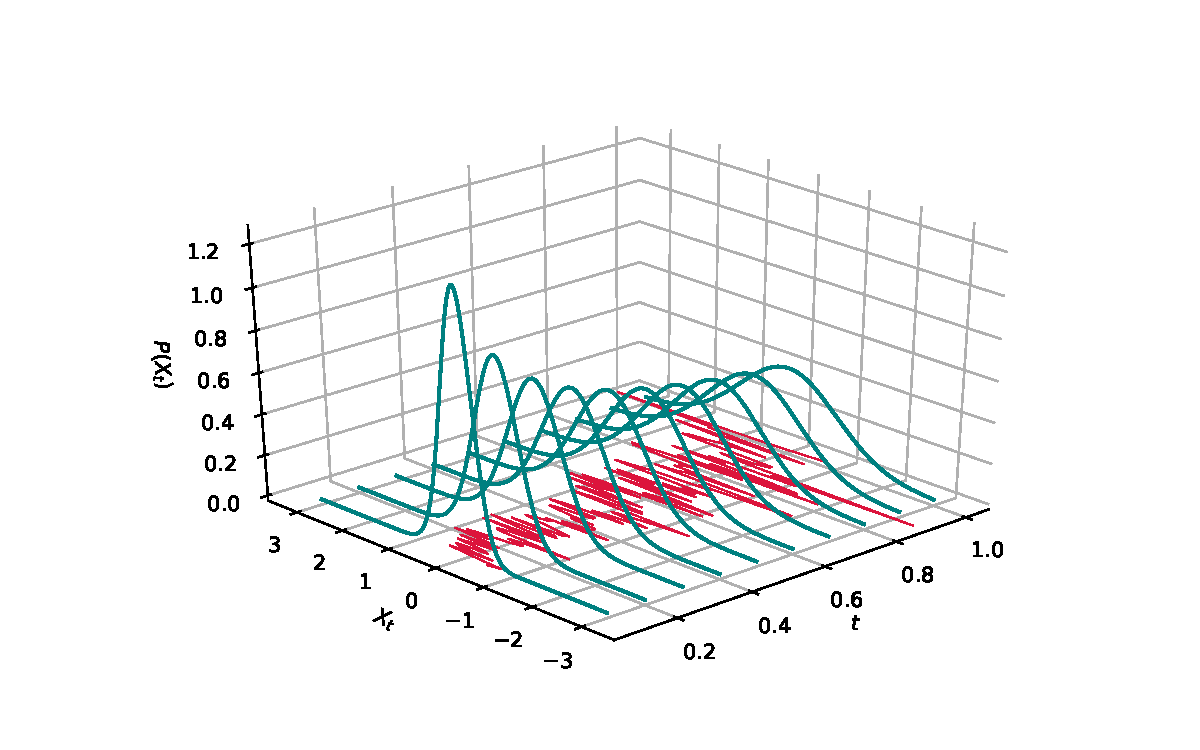
\includegraphics[width=0.90\textwidth]{../images/stoch_process_3d}
	\caption{Distribution and Path of a Stochastic Process.}
	\label{fig:stochastic_process}
\end{figure}

Consider figure \ref{fig:stochastic_process}, where we graph a single path of the stochastic process $\ctspr$ in which $X_t \sim \mathcal{N}(0, t)$ (see eq. \ref{eq:normal_distribution}). Indeed, $\ctspr$ can be seen as either a function indexed by $T$, in which case we graph the path of a single trajectory (red colored); or, for fixed $t\geq 0$, as a single random variable with probability density function $\phi(x | 0, t)$.\\

With stochastic processes well defined, the next step is to measure the outcome of an event at a given $t \geq 0$. Unlike this last example, stochastic processes need not be $\borelsalg$-measurable for every $t$. The values that any $\ctspr$ can take at a certain $t$ may vary. For this reason, it is sensible to equip a stochastic process, with $\salg$s of subsets of $\salgF$ that give us clue as to the subsets that are \textit{reasonable} to measure at a given $t$. 

\begin{definition}[\textbf{Filtration}]
Let $\ProbSpace$ a probability space. A filtration is a non-decreasing sequence of sub-$\salg$s of $\salgF$, $\{\salgF_n\}_{n\geq 0}$ such that 
\[
	\salgF_t \leq \salgF_s \ \forall \ 0 \leq t \leq s.
\]
\end{definition}

The stochastic process $\ctspr$ is said to be \textbf{adapted} to the filtration $\{\salgF_t\}_{t\geq 0}$ if $X_t$ is $\salgF_t$-measurable for every $t\geq 0$.\\

The minimal $\salg$ generated by $\ctspr$ at time $\tau$ is known as the \textbf{natural filtration} of $\ctspr$ at time $\tau$. Note that $\ctspr$ is always adapted to its natural filtration at time $t$. That is $X_t$ is $\sigma(\{X_s | s \leq t\})$-measurable.\\

In a discrete time process, we denote the minimal $\salg$ generated by $\dtspr$ up to time $k$ as $\{X_1, \ldots, X_k\} := \sigma(\{X_1, \ldots, X_k\})$.\\

We conclude this chapter by defining a particular subset of the family of stochastic processes. We will limit ourselves to define it here and develop its intuition in the following chapter.

\begin{definition}[\textbf{Martingale}]\label{def:martingale}
	A stochastic process $\ctspr$ defined over $\ProbSpace$ is said to be a martingale w.r.t. a filtration $\{\salgF_n\}_{n\geq 0}$ if, for all $0 \geq s \leq t$,
	\begin{enumerate}
		\item $X_t$ is $\salgF_t$-measurable;
		\item $X_t$ is in $L_1$ (i.e. is is measurable for all $t$); and
		\item $\E[X_t | \salgF_s] = X_s$.
	\end{enumerate}
\end{definition}

\begin{theorem}[\textbf{Doob's Martingale Inequality}]\label{th:doob_martingale}
	If. $\ctspr$ is a continuous-time martingale, then 
	\begin{equation}
		\Pm(\sup_{t\in [0, T]} |X_t| \geq \lambda) \leq \frac{1}{\lambda^p}\E\left[|X_t|^p\right].
	\end{equation}
	
\end{theorem}

	
\end{document}